\documentclass[11pt]{article}

\usepackage[margin=1in]{geometry}
\usepackage{amsmath, amssymb}
\usepackage{graphicx}
\usepackage[numbers,sort&compress]{natbib}
\usepackage{xurl}
\usepackage{hyperref}

\title{Supplementary Note: Popcount as Hamming Weight and an Entropy-Oriented Diagnostic}
\author{Simon Tian}
\date{}

\begin{document}

\maketitle

\begin{abstract}
This review-only supplement reframes the popcount-based Gaussianization
argument in information-theoretic language. The main point is that popcount,
more formally the Hamming weight, is an entropy-related diagnostic of
first-order bit balance rather than a complete standalone quality measure for a
random number generator. Matching the ideal Hamming-weight law is therefore
useful evidence, but it does not by itself rule out dependence, structural
artifacts, or predictability in the underlying source.
\end{abstract}

\section{Review Status}

This note is intended as a standalone supplement for internal review before any
material is merged into the main manuscript. It leaves the main paper
unchanged and instead collects one alternative interpretation of the current
popcount analysis.

\section{Popcount as Hamming Weight}

Let $X = (X_1,\dots,X_n) \in \{0,1\}^n$ be an $n$-bit output and define its
Hamming weight
\[
W_n = \sum_{i=1}^n X_i.
\]
In the manuscript, $W_n$ is the popcount of a VM-native output. Under an ideal
unbiased independent-bit model, $X_i \sim \mathrm{Bernoulli}(1/2)$ and
\[
W_n \sim \mathrm{Binomial}(n,1/2).
\]
Under the broader heterogeneous-bit model already used in the main paper,
$W_n$ is Poisson-binomial instead \citep{Hong2013}. The central-limit-theorem
argument in the manuscript then explains why the standardized Hamming weight is
close to Gaussian under mild regularity conditions \citep{Durrett2019}.

This perspective is useful because it isolates a specific question about the
generator: do the bits appear balanced enough that the empirical weight law
looks like the law predicted by fair coin flips?

\section{An Entropy Decomposition}

The information-theoretic interpretation comes from the fact that the Hamming
weight identifies only the \emph{composition} of the bit string, not the
arrangement of the $1$'s inside it. For a fixed weight $w$, the number of
binary strings having exactly $w$ ones is
\[
\binom{n}{w}.
\]
Conditioned on $W_n = w$, the remaining uncertainty is the choice of which $w$
positions carry the ones, so
\[
H(X \mid W_n = w) = \log_2 \binom{n}{w}.
\]
This yields the standard entropy decomposition
\[
H(X) = H(W_n) + H(X \mid W_n).
\]

The consequence is immediate: the Hamming-weight variable compresses the
original $n$-bit output very aggressively. For unbiased independent bits,
$H(X)=n$ bits, whereas $H(W_n)$ grows only on the order of $\log n$. At the
digest width used throughout much of the paper,
\[
H(W_{256}) \approx 5.05 \text{ bits},
\]
while the full $256$-bit output has $256$ bits of Shannon entropy under the
ideal model.

So the Hamming-weight distribution is entropy-related, but only in a narrow
sense: it measures whether the aggregate bit-balance behavior is compatible
with high-entropy fair-coin outputs. It does \emph{not} retain the full
information content of the underlying string.

\section{What This Means for RNG Quality}

This provides an alternative interpretation of the current manuscript figures.
The popcount diagnostics test whether the generator looks correct at a
first-order level:
\begin{itemize}
\item are the bits centered near a fair split between zeros and ones?
\item do the empirical weight probabilities follow the expected
binomial/Poisson-binomial shape?
\item do the quantiles and tails materially deviate from the ideal reference?
\end{itemize}

Those are meaningful quality checks, but they are not exhaustive. A generator
can have a convincing Hamming-weight distribution and still be deficient in
other ways: short-period structure, lag dependence, repeated patterns, or
cryptographic predictability may still remain. That is why the Hamming-weight
view is best read as a \emph{first-order marginal diagnostic}, not as a full
randomness certification. This is consistent with the broader philosophy behind
local statistical batteries such as NIST SP 800-22, where useful statistical
tests are treated as diagnostics rather than complete certification by
themselves \citep{NISTSP80022}.

For that reason, an entropy-oriented framing should strengthen rather than
replace the current evaluation logic. A practical interpretation is:
\begin{enumerate}
\item the Hamming-weight law checks bit balance and aggregate distributional fit;
\item dependence diagnostics such as repeated-sequence ACF remain necessary,
because they probe structure not visible after reducing each output to a single
weight;
\item if a scalar entropy-flavored score is desired, a cleaner candidate is the
Kullback--Leibler divergence between the empirical weight law and the ideal
reference law,
\[
D_{\mathrm{KL}}(\widehat{P}_{W_n} \,\|\, P_{W_n}^{\star})
=
\sum_w \widehat{P}_{W_n}(w)
\log \frac{\widehat{P}_{W_n}(w)}{P_{W_n}^{\star}(w)},
\]
where $P_{W_n}^{\star}$ is the ideal binomial or Poisson-binomial reference.
\end{enumerate}

\section{Connection to the Current Origin Figures}

Figures~\ref{fig:cdf}--\ref{fig:acf} show how the entropy-oriented reading maps
onto the refreshed Origin exports. The first three figures diagnose the
Hamming-weight law directly, while the final figure shows why a separate
dependence check is still needed.

\begin{figure}[htbp]
\centering
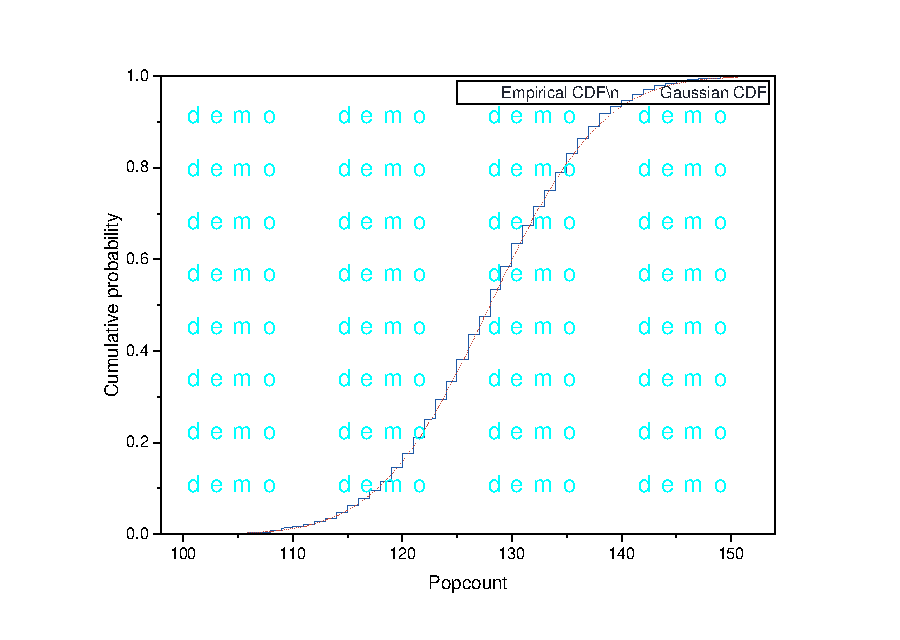
\includegraphics[width=0.72\linewidth]{origin_package/origin_exports/popcount_cdf_origin.pdf}
\caption{Empirical Hamming-weight CDF against the Gaussian/binomial-style
reference. In the entropy-oriented reading, this figure checks whether the
aggregate weight law is centered and shaped as expected under near-fair bit
balance.}
\label{fig:cdf}
\end{figure}

\begin{figure}[htbp]
\centering
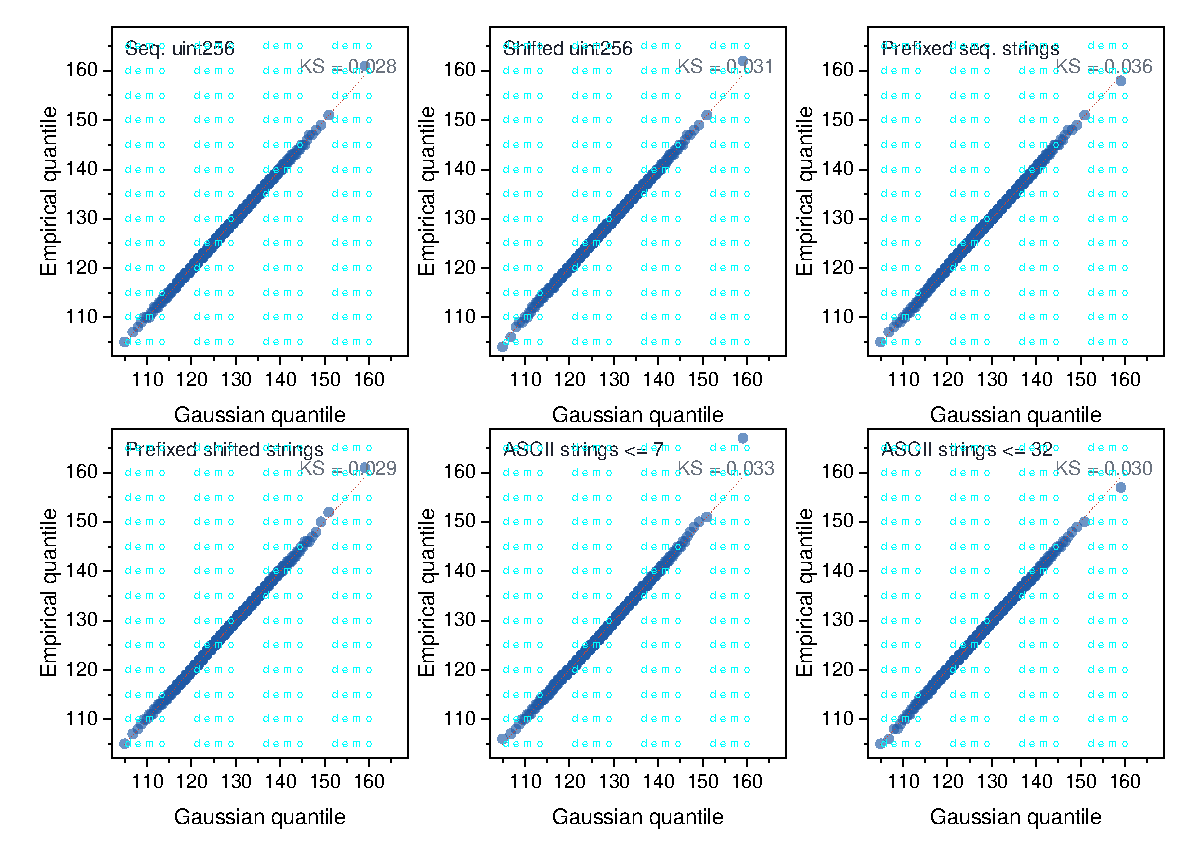
\includegraphics[width=\linewidth]{origin_package/origin_exports/popcount_qq_panels_origin.pdf}
\caption{Hamming-weight quantile alignment across experiments. These panels are
best read as a check on whether the observed type-class mass accumulates in the
same way as the ideal reference law.}
\label{fig:qq}
\end{figure}

\begin{figure}[htbp]
\centering
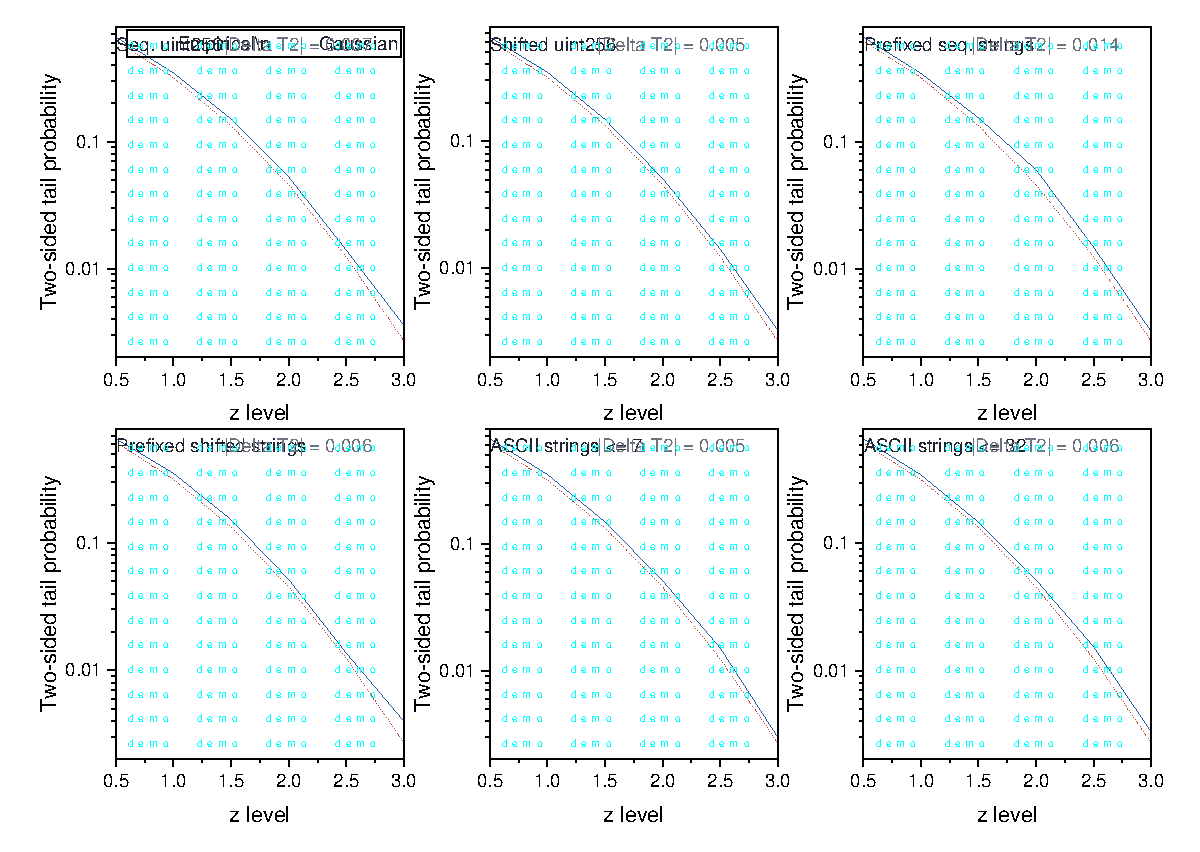
\includegraphics[width=\linewidth]{origin_package/origin_exports/popcount_tail_panels_origin.pdf}
\caption{Hamming-weight tail probabilities across experiments. Tail behavior is
important because it detects whether the generator allocates too much or too
little probability to unusually light or unusually heavy outputs.}
\label{fig:tail}
\end{figure}

\begin{figure}[htbp]
\centering
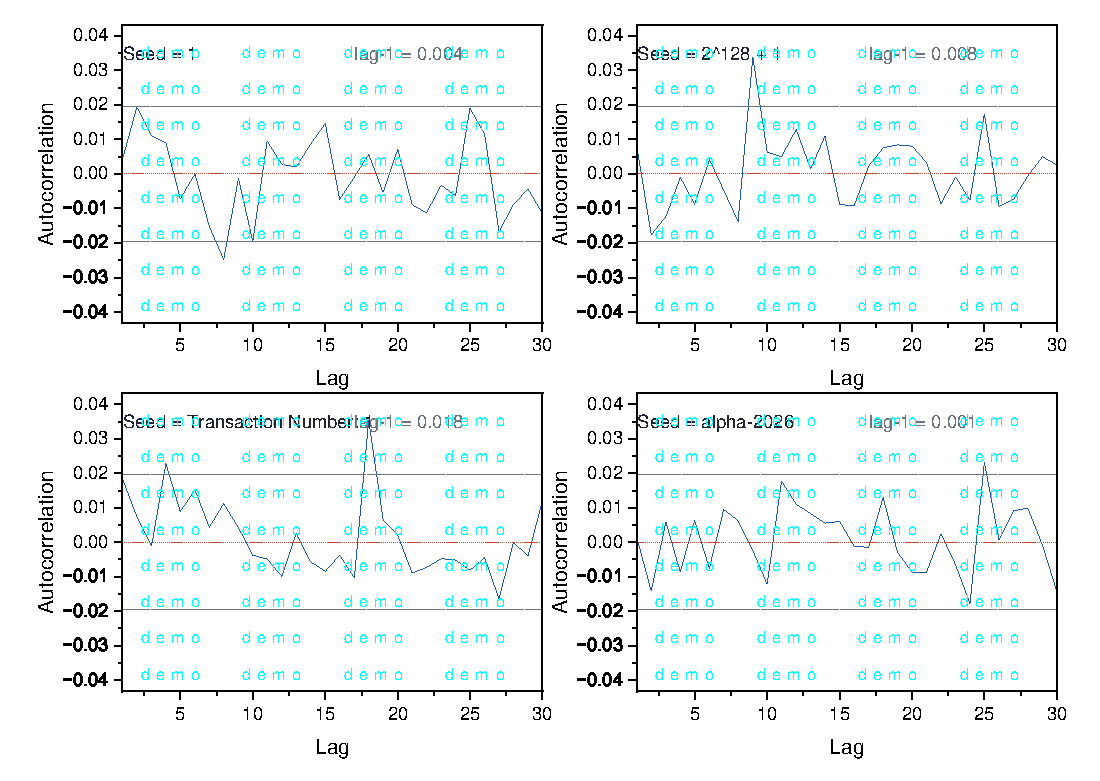
\includegraphics[width=0.92\linewidth]{origin_package/origin_exports/sequence_acf_panels_origin.pdf}
\caption{Repeated-sequence autocorrelation panels. This figure is not a
Hamming-weight diagnostic; it is included to emphasize that good weight-law fit
does not by itself rule out lag dependence or sequence structure.}
\label{fig:acf}
\end{figure}

\section{Suggested Positioning}

If any of this is merged into the main manuscript, the cleanest claim is the
following:

\medskip
\noindent
\emph{The Hamming-weight distribution is an entropy-related indicator of
marginal bit balance, but it is not by itself a complete quality measure for
the underlying random number generator.}
\medskip

That wording preserves the value of the current popcount analysis while making
its scope explicit.

\bibliographystyle{plainnat}
\bibliography{references}

\end{document}
